%UCA-3: Configura Server

\begin{figure}
\centering
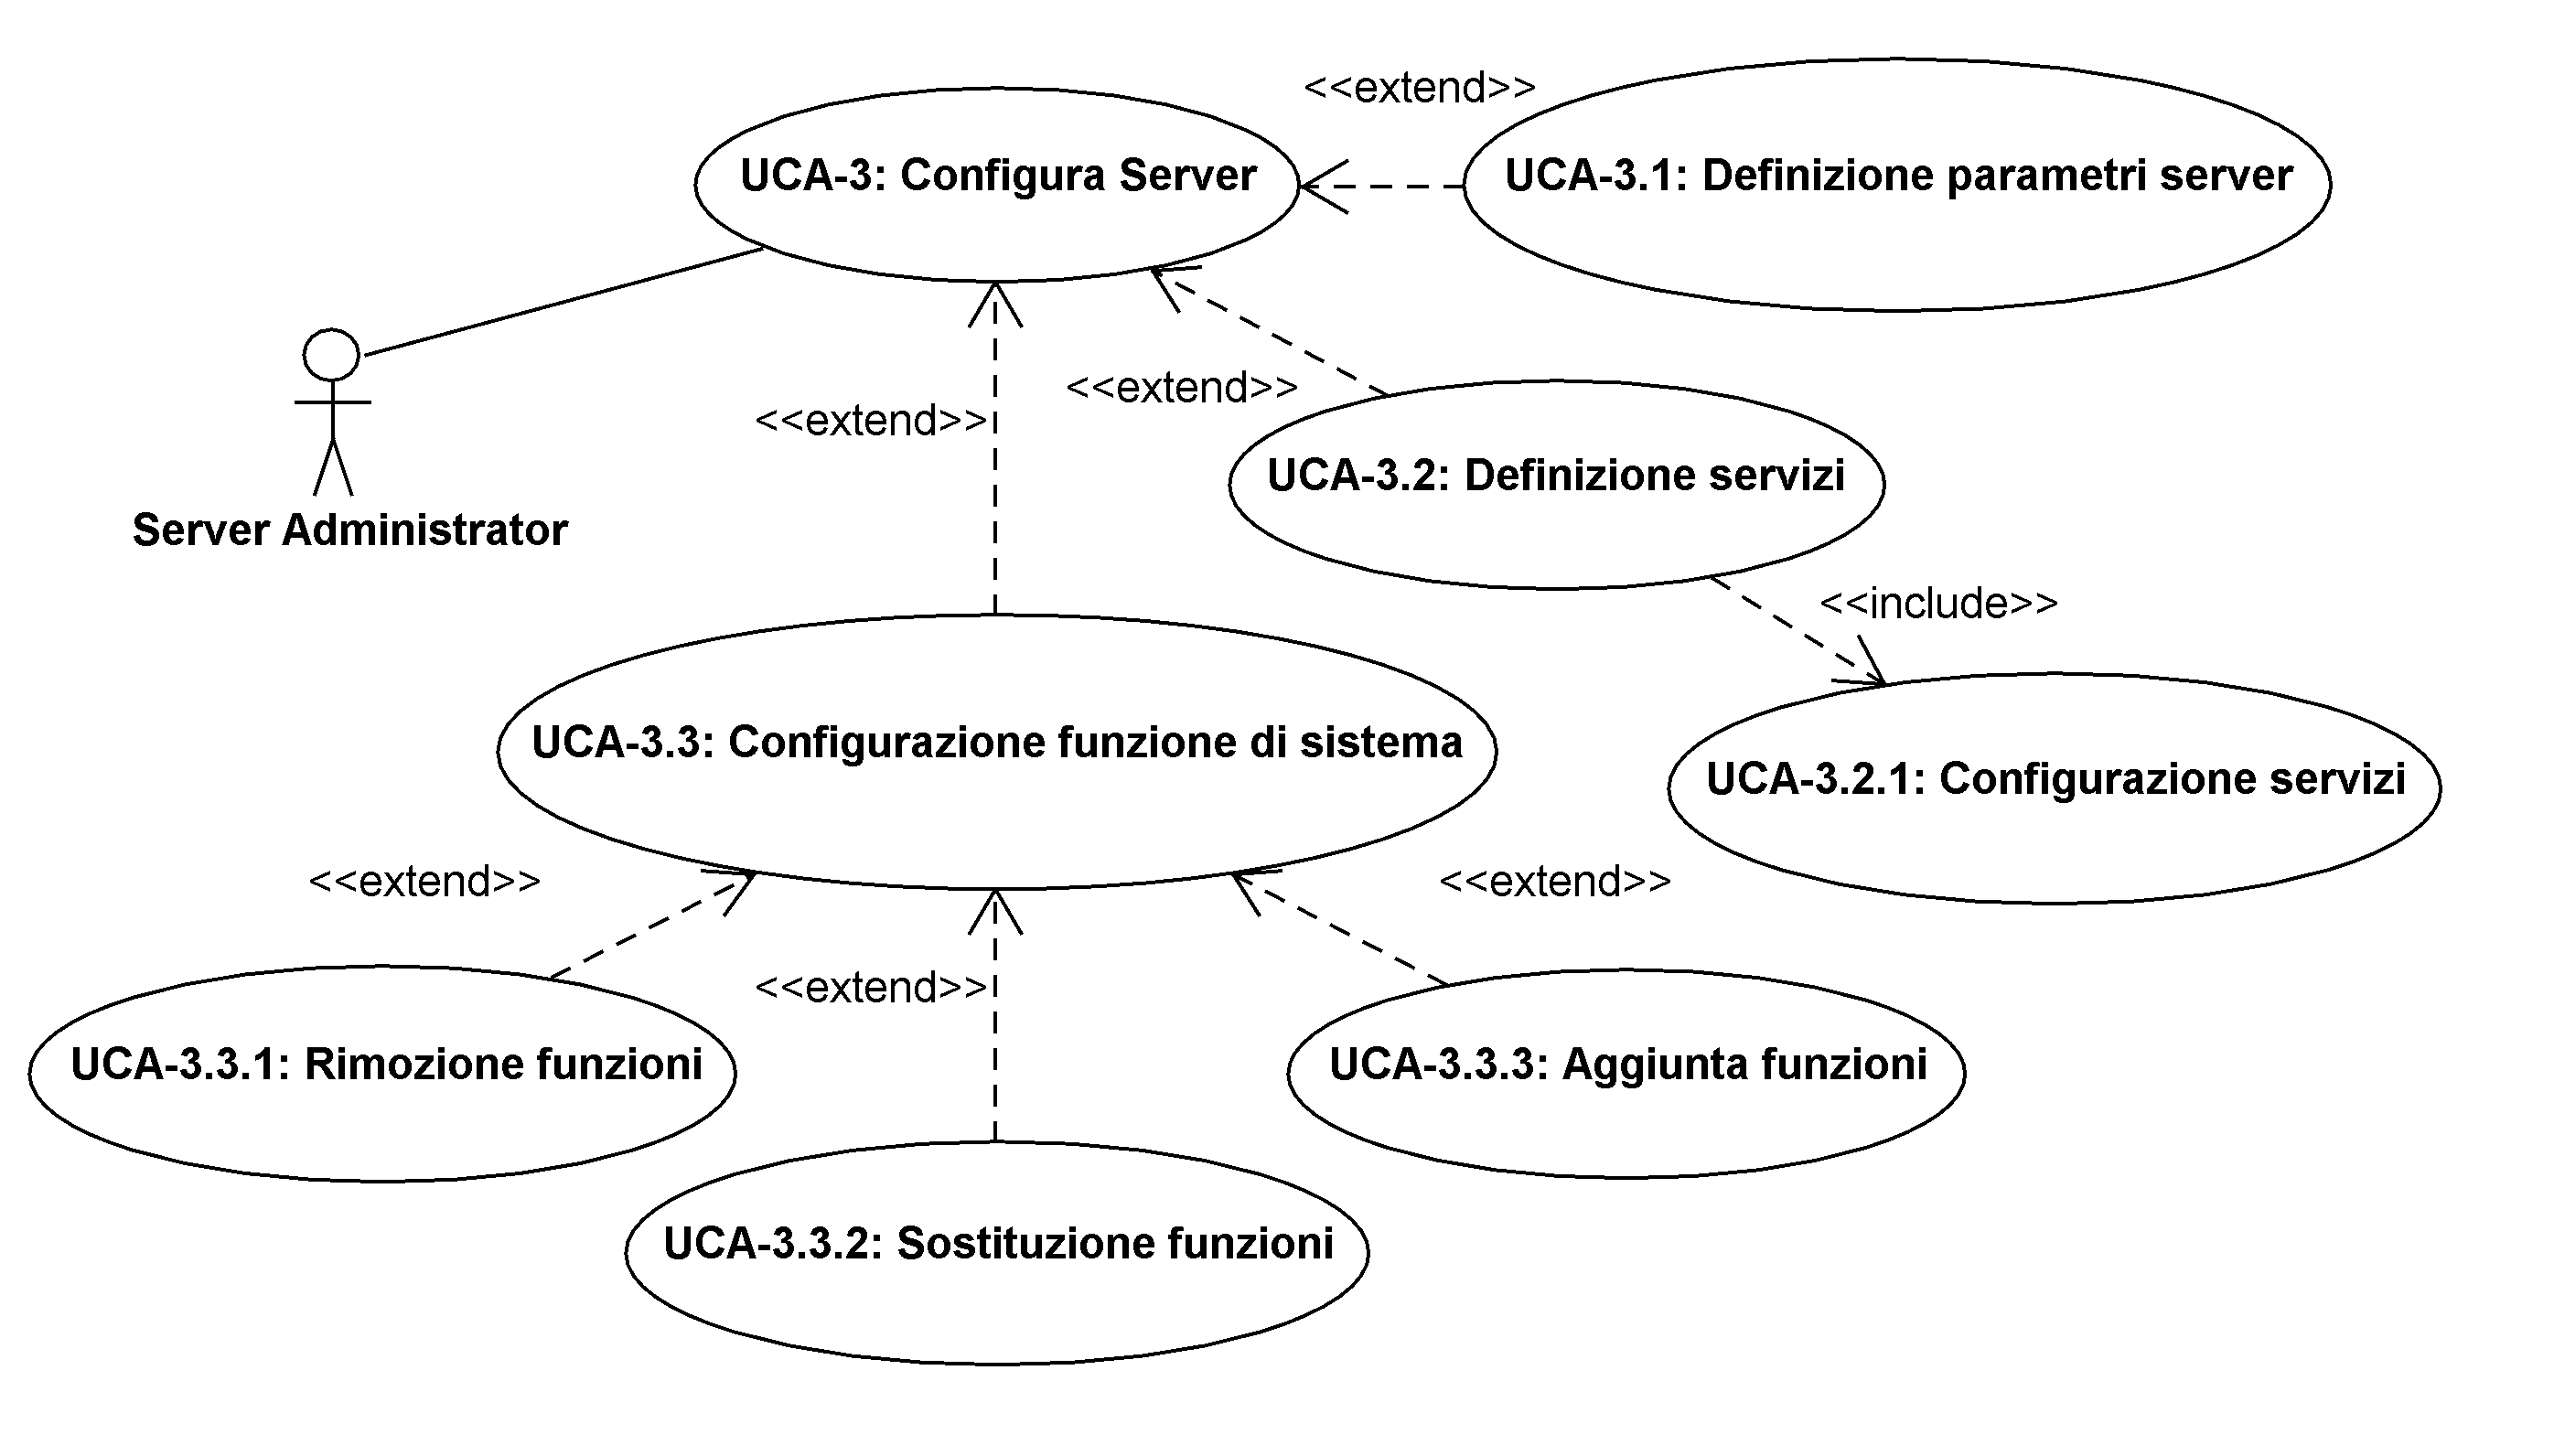
\includegraphics[width=1.1\textwidth]{Immagini/Capitolo2/UseCases/UCA-3.png}
\caption{Diagramma dei casi d'uso UCA-3}\label{fig:uc-uca-3}
\end{figure}

\begin{itemize}
	\item \textbf{Attori:} Server Administrator
	\item \textbf{Scopo e descrizione:} il Server Administrator deve avere la possibilità di configurare le funzioni del software MyCLIPS utilizzabili dai client, i servizi offerti dal server e i parametri di base del modulo server attraverso un file di configurazione
	\item \textbf{Pre-condizioni:} il sistema offre un formato di specifica delle configurazioni e un meccanismo di caricamento delle stesse
	\item \textbf{Post-condizioni:} il funzionamento del software rispecchia i parametri definiti del file di configurazione
	\item \textbf{Flusso principale degli eventi:}
		\begin{enumerate}
			\item il Server Administrator apre il file di configurazione attraverso un programma di \emph{text-editing}
			\item il Server Administrator modifica i parametri di configurazione del server
				\begin{itemize}
					\item il Server Administrator modifica le funzioni di MyCLIPS utilizzabili dai client (si guardi il caso d'uso \emph{UCA-3.3})
					\item il Server Administrator modifica i servizi attivi offerti dal server (si guardi il caso d'uso \emph{UCA-3.2})
					\item il Server Administrator modifica modifica i parametri di base del server (si guardi il caso d'uso \emph{UCA-3.1})
				\end{itemize}
			\item il Server Administrator salva le modifiche
		\end{enumerate}
\end{itemize}


\paragraph{UCA-3.1: Configurazione parametri server}

\begin{itemize}
	\item \textbf{Attori:} Server Administrator
	\item \textbf{Scopo e descrizione:} il Server Administrator deve avere la possibilità di modificare i parametri di configurazione di base del server
	\item \textbf{Pre-condizioni:} \emph{nessuna}
	\item \textbf{Post-condizioni:} i parametri di configurazione risultano modificati secondo le aspettative del Server Administrator
	\item \textbf{Flusso principale degli eventi:}
		\begin{enumerate}
			\item il Server Administrator modifica i parametri di base del server. Può configurare:
				\begin{itemize}
					\item l'indirizzo di ascolto (\emph{bind-address})
					\item la porta di ascolto (\emph{bind-port})
					\item la creazione di un registro delle richieste (\emph{log-requests})
					\item il livello di dettaglio del registro delle richieste (\emph{log-level})
				\end{itemize}
		\end{enumerate}
\end{itemize}


\paragraph{UCA-3.2: Definizione servizi}

La descrizione comprende anche quella del caso d'uso \emph{UCA-3.2.1}.

\begin{itemize}
	\item \textbf{Attori:} Server Administrator
	\item \textbf{Scopo e descrizione:} il Server Administrator deve avere la possibilità di definire i servizi attivi offerti dal server e configurare i parametri di funzionamento dei servizi
	\item \textbf{Pre-condizioni:} \emph{nessuna}
	\item \textbf{Post-condizioni:} i parametri di configurazione risultano modificati secondo le aspettative del Server Administrator
	\item \textbf{Flusso principale degli eventi:}
		\begin{enumerate}
			\item il Server Administrator modifica i servizi attivi offerti dal server specificando:
				\begin{itemize}
					\item l'interfaccia offerta dal servizio
					\item un'implementazione del servizio
				\end{itemize}
			\item il Server Administrator specifica i parametri relativi ai servizi attivi (\emph{UCA-3.2.1)}: il formato, il tipo e i valori delle configurazioni sono definite dalla specifica implementazione del servizio
		\end{enumerate}
\end{itemize}





